\begin{frame}
	\frametitle{Disconnect, Privacy Badger (EFF), Ghostery}

	\begin{center}
		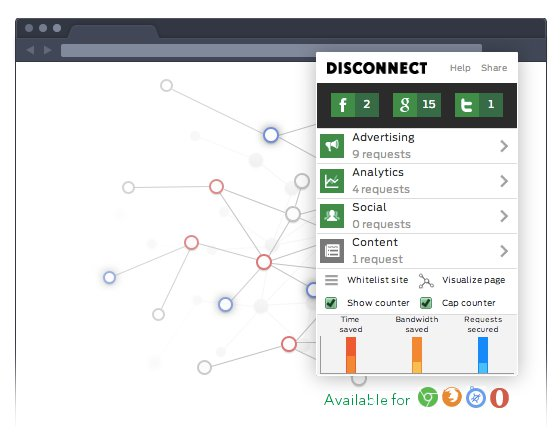
\includegraphics[height=0.7\textheight]{../../img/disconnectme.jpg}
	\end{center}
\end{frame}
\note{Auf dem PC und Laptop ist das vorgehen gegen Tracking leicht. Es gibt Addons für Chrome, Firefox etc.\ die Webseiten die Kommunikation mit Trackern einfach verbieten. Disconnect und Privacy Badger sind dabei Open Source und sollten wenn möglich dem bekannteren Ghostery vorgezogen werden.}

\begin{frame}
	\frametitle{Android: Antitracking im Firefox Privatmodus}

	\begin{center}
		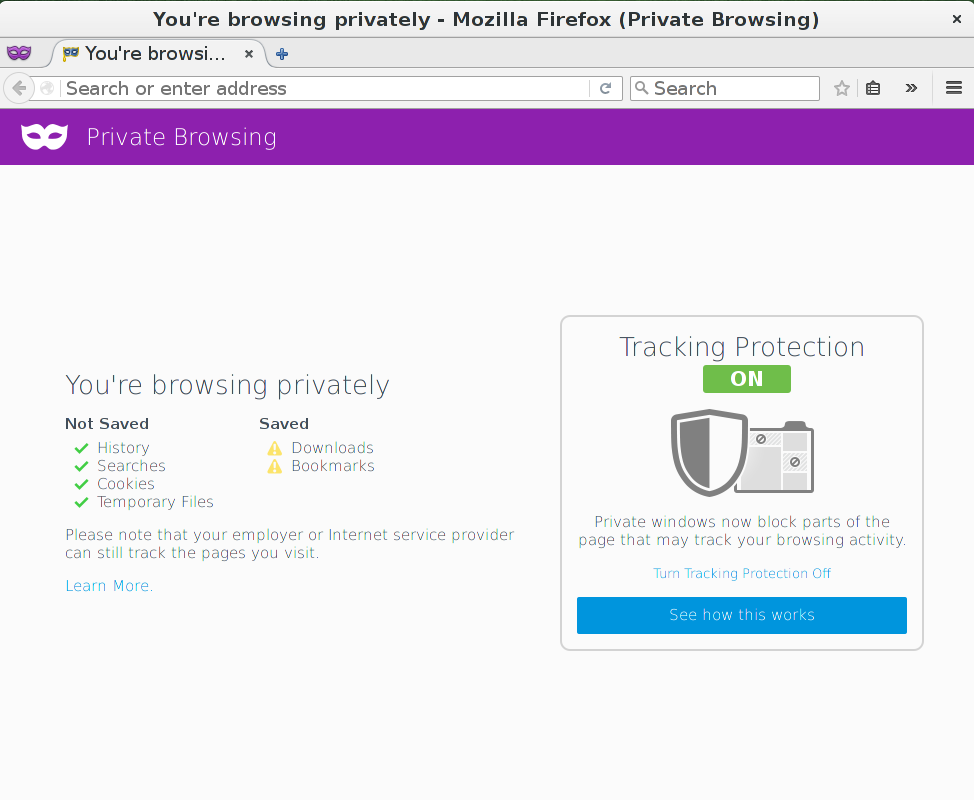
\includegraphics[height=0.7\textheight]{../../img/ff_antitrack.png}

    \textbf{Installation für Firefox auf Android}\\
		Firefox-Menü -> Extras -> Add-ons -> Alle Firefox-Addons ansehen -> nach Tracking suchen -> "Enable Tracking Protection" installieren.
	\end{center}
\end{frame}
\note{Auch der Privatmodus im Firefox kann mittlerweile Tracking verbieten. Er benutzt dafür die Sperrliste von Disconnect. Aber eines der Addons nutzen ist trotzdem besser, weil das dann auch im normalen Modus funktioniert. Alternativ kann man als Firefox-Benutzer auch das Addon ``Enable Tracking Protection'' benutzen, dann ist der eingebaute Trackingschutz immer aktiv - das geht auch unter Android!}

\begin{frame}{Antitracking im mobilen Firefox}
	\begin{columns}
		\column{5.5cm}
		\footnotesize
		\textbf{ab Firefox 58}\\
		Einstellungen -> Datenschutz -> Schutz vor Aktivitätenverfolgung\\
		\vspace{0.5cm}

		\column{5cm}

		\begin{center}
			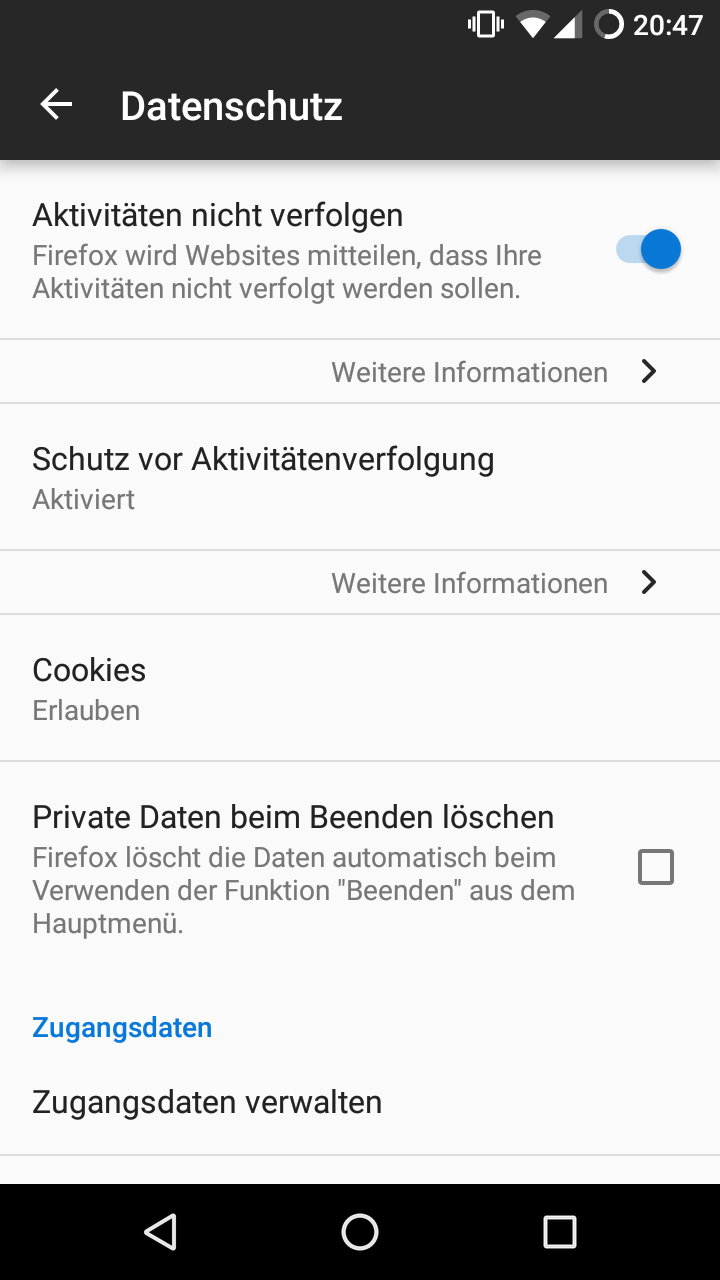
\includegraphics[width=3.5cm]{../../img/firefox-mobil-antitracking.png}
		\par\end{center}
	\end{columns}
\end{frame}
\note{Bei neueren Firefox Mobilversionen kann man das Antitracking in den Einstellungen explizit anschalten}

\begin{frame}
	\frametitle{Antitracking Browser für iOS: Firefox Klar}

	\begin{center}
		
\includegraphics[height=0.5\textheight]{../../img/firefox-klar.jpg}
	\end{center}
\end{frame}
\note{Blockiert Werbung und verhindert Tracking!}

\begin{frame}{Antitracking für mobile Apps}
	\begin{columns}
		\column{5.5cm}
		\footnotesize
		\textbf{Android: Google AdID}\\
		Google-Einstellungen -> Anzeigen -> Interessensbezogene Werbung deaktivieren\\
		\vspace{0.5cm}

		\textbf{iOS: Apple IDFA}\\
		Einstellungen -> Datenschutz -> Werbung -> Kein Ad-Tracking\\
		\vspace{0.5cm}

		\column{5cm}

		\begin{center}
			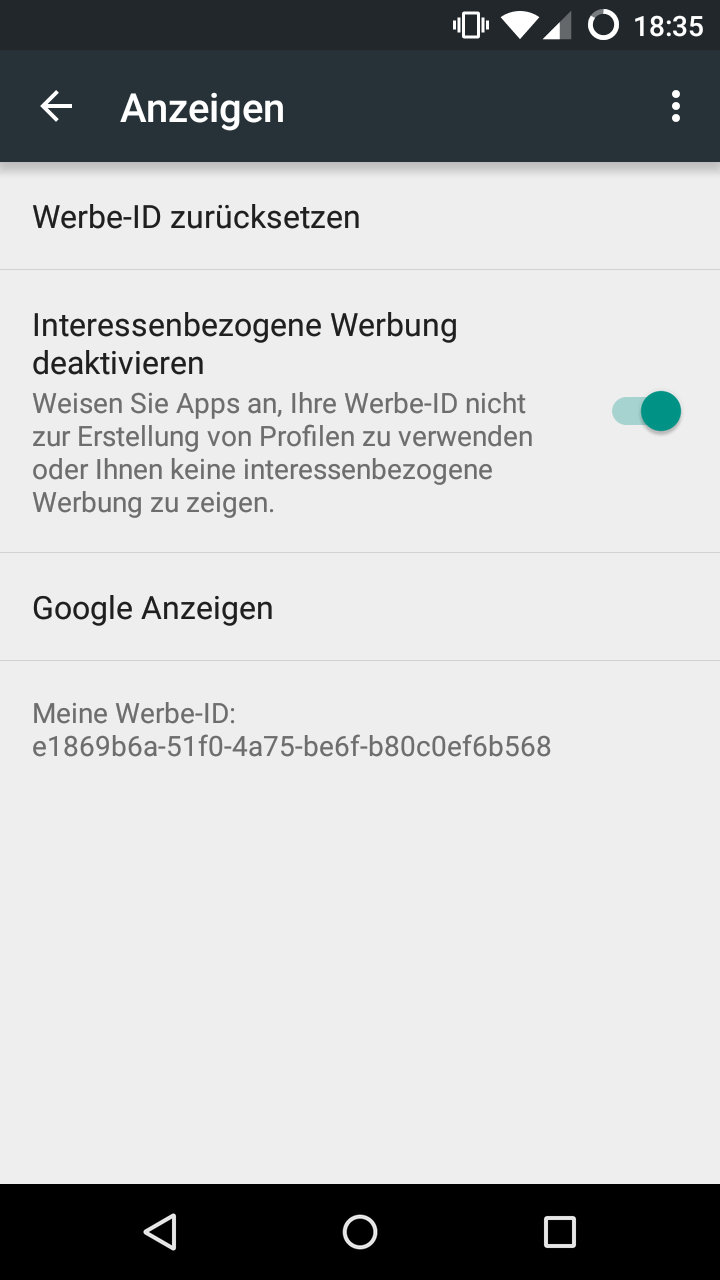
\includegraphics[width=3.5cm]{../../img/google-adid.png}
		\par\end{center}
	\end{columns}
\end{frame}
\note{Bei mobilen Apps kann man das Tracking zentral für alle verbieten. Das liegt daran, dass auf iOS und Android den Apps das Tracken nur mit einer von Apple oder Google für jeden Nutzer vergebenen, eindeutigen ID erlaubt ist. Diese kann man wie auf der Folie gezeigt deaktivieren.}
